


\documentclass[
footnotes=multiple,
parskip=half,
numbers=noendperiod
]{scrartcl}

\usepackage[ngerman]{babel}
\usepackage[utf8]{inputenc}
\usepackage[T1]{fontenc}
\usepackage{ulem}
\usepackage{pdfpages}
\usepackage{hyperref}

\author{Wolfgang Niedermayr}

\title{Paternoster SPS-Programm}
\begin{document}
%\maketitle %
%\tableofcontents
\begin{center}
	\Huge{\bfseries{Lagersystem \\SPS-Programm\\}}
\end{center}
~%
\\%
\\%
~%
\huge{\bfseries{Inhaltsverzeichnis\\}%
\small Es sind nur die wichtigsten Bausteine angeführt.\\~\\%

\begin{enumerate}

	\item {\hyperlink{GlobDB.1}{Globaler Daten DB}}
	\item {\hyperlink{Ob1.1}{OB 1}}
	\item {\hyperlink{Inp.1}{Inputs}}
	\item {\hyperlink{FrgBa.1}{Freigaben und Betriebsarten}}
%	\item {\hyperlink{HMISS.1}{Schnittstelle des HMI Bausteins}}
	\item {\hyperlink{HMI.1}{HMI Baustein}}	
	\item {\hyperlink{Lager.1}{Lager Baustein}}	
%	\item {\hyperlink{OutSS}{Schnittstelle Outputs}}
	\item {\hyperlink{Out}{Outputs Baustein}}
\end{enumerate}

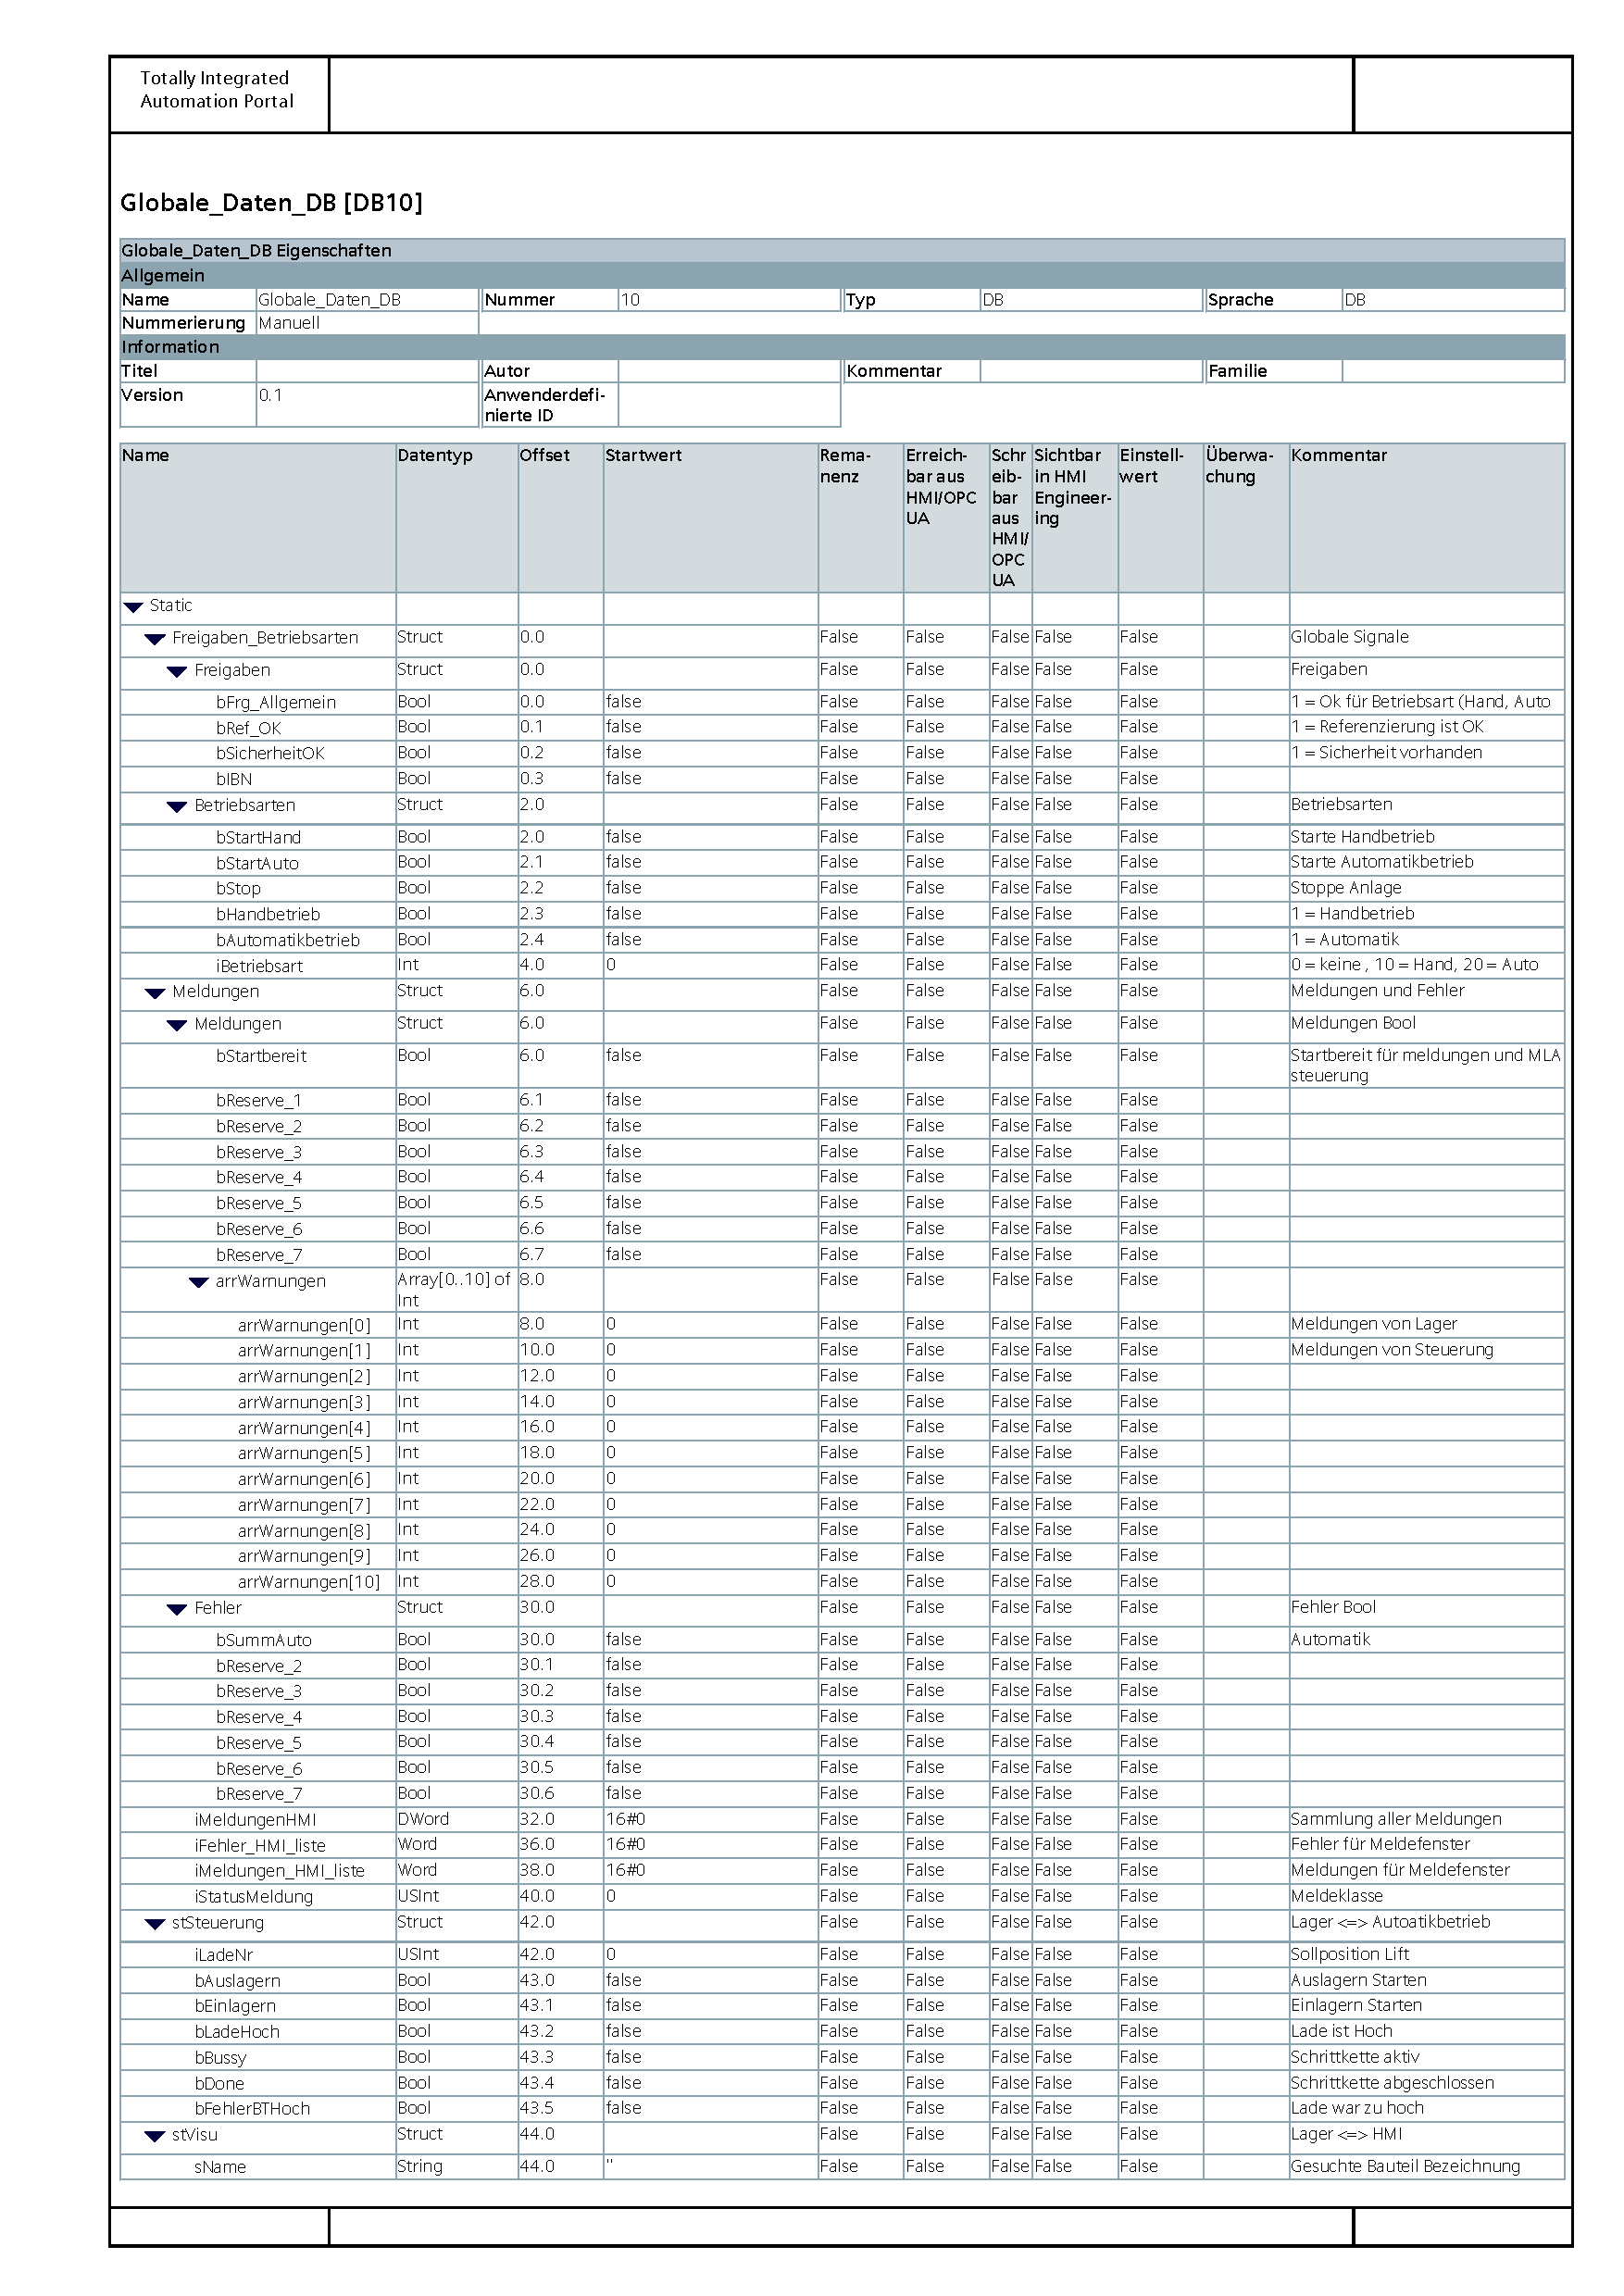
\includepdf[scale=0.8,pages=-,link=true,linkname=GlobDB]{../PROGRAMM/EinzelnePdfs/GlobaleDaten_DB10.pdf}
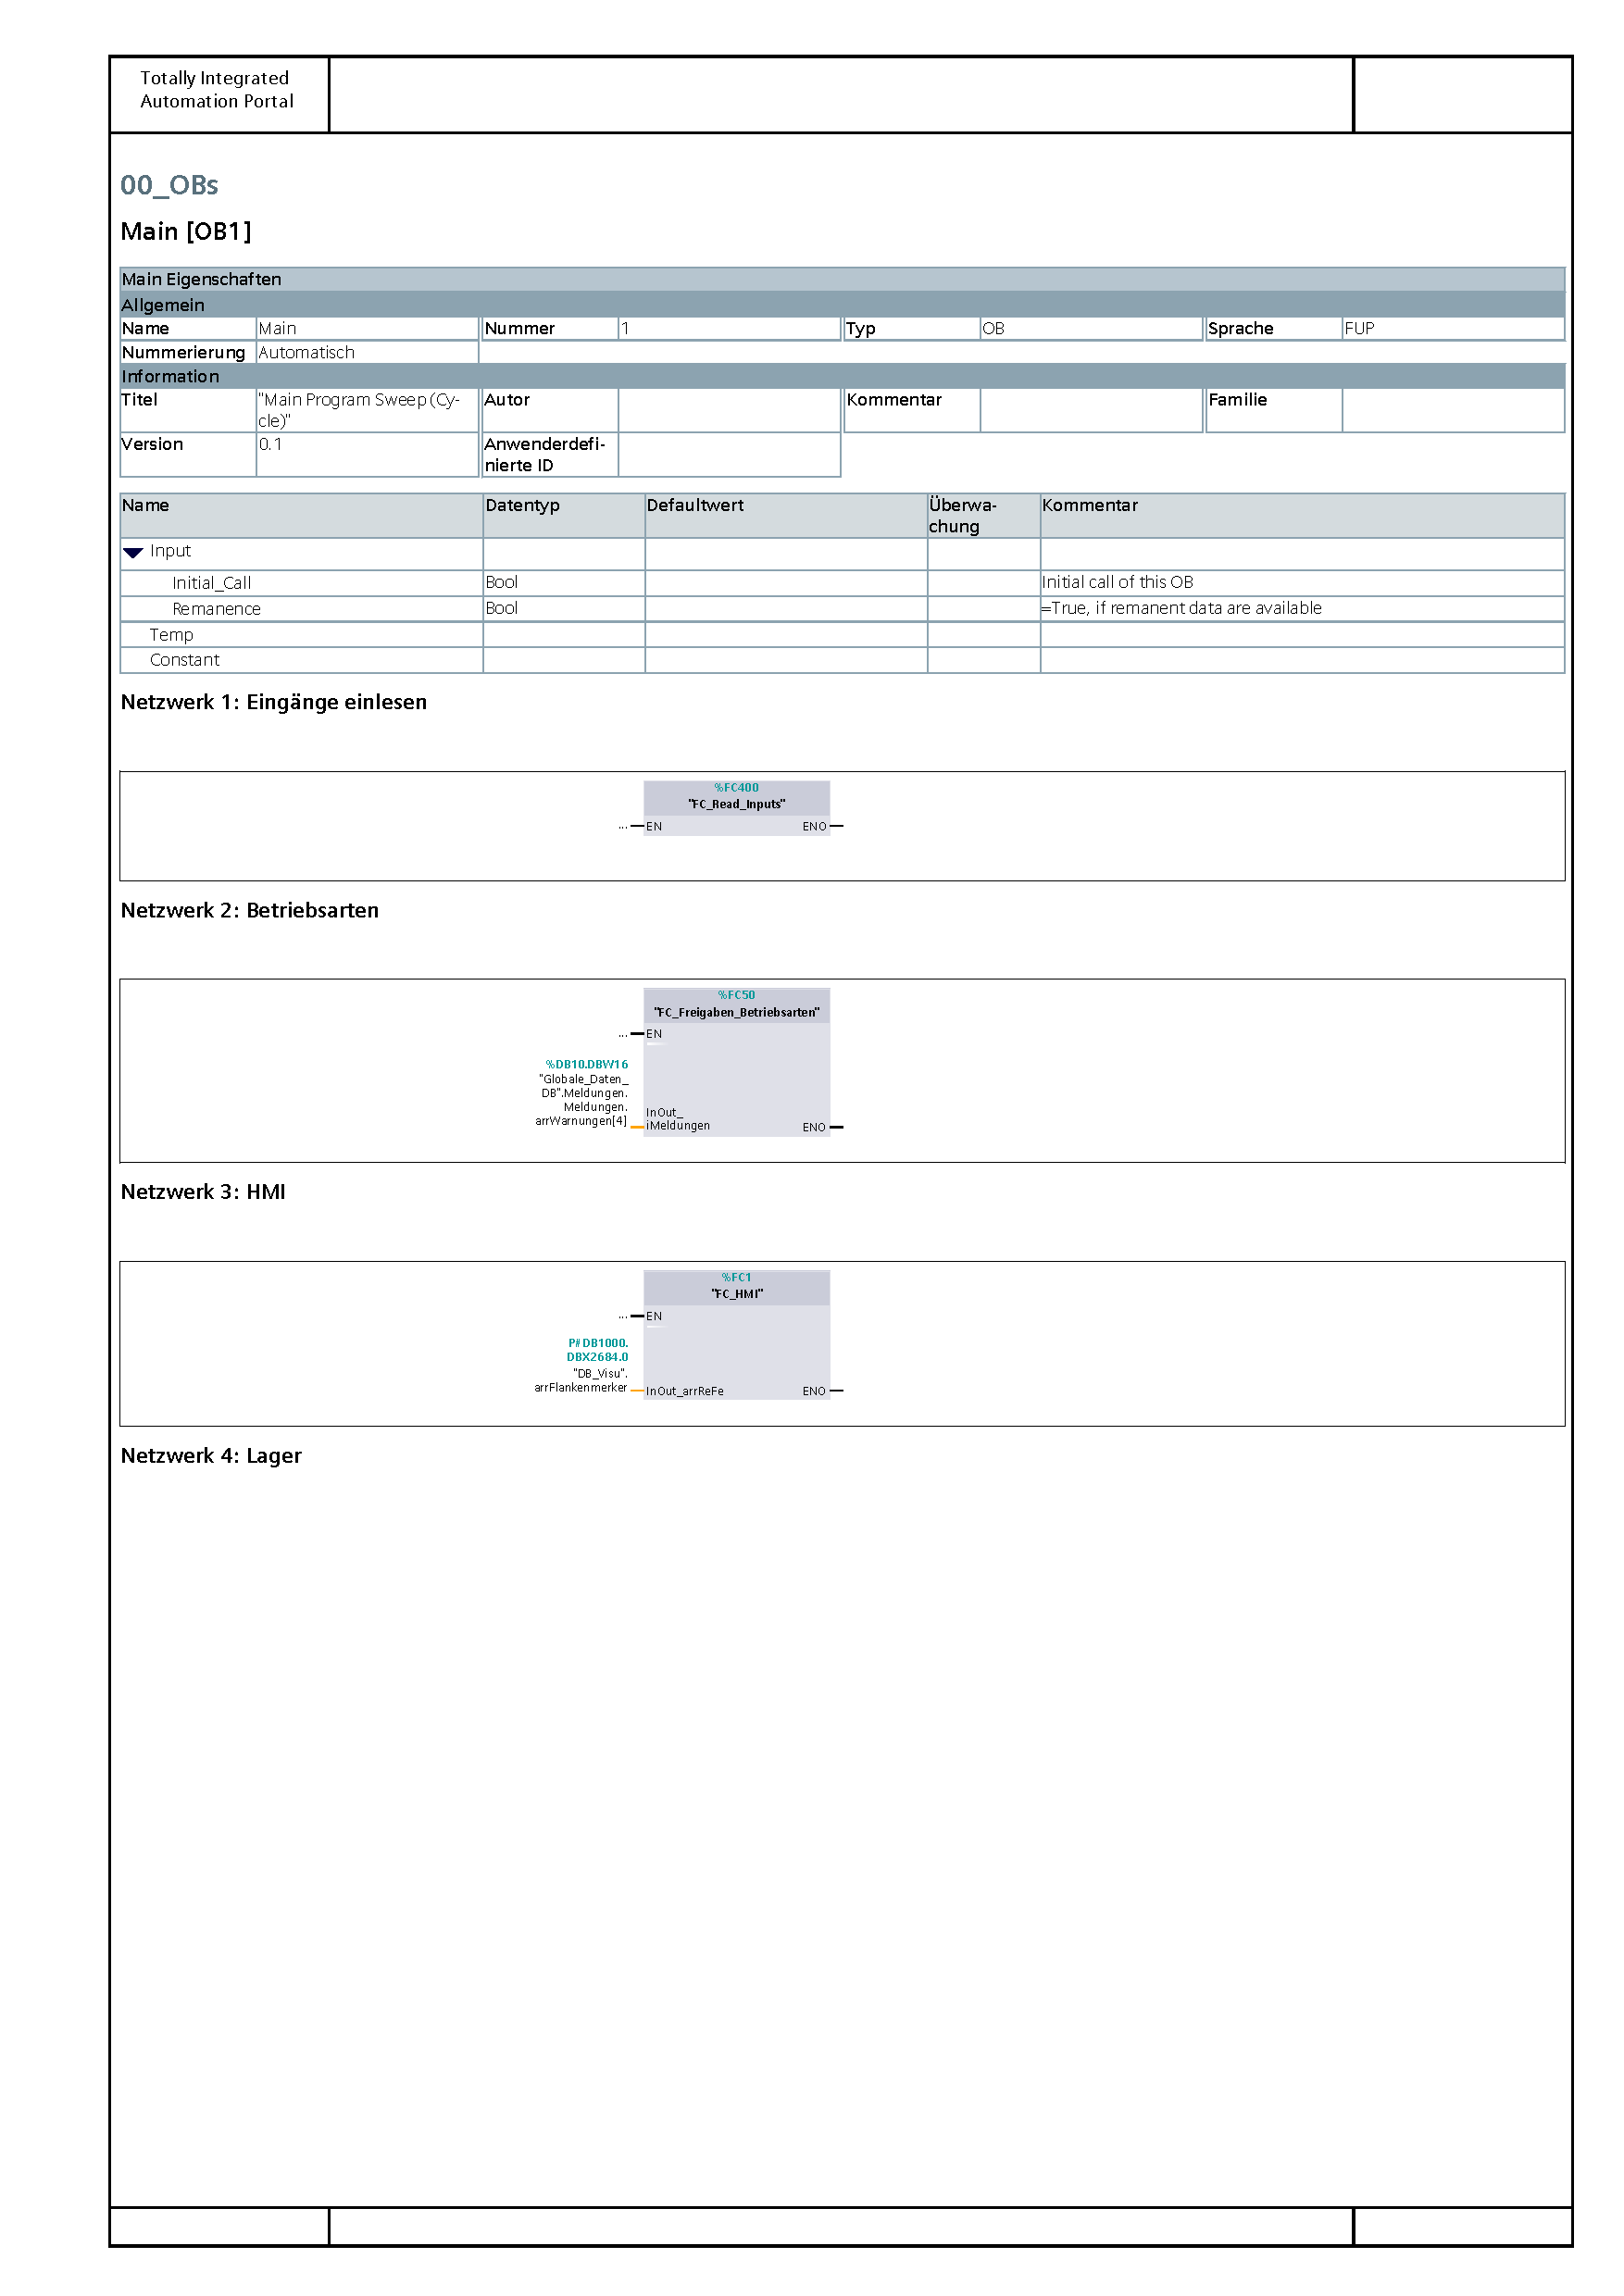
\includepdf[scale=0.8,pages=-,link=true,linkname=Ob1]{../PROGRAMM/EinzelnePdfs/OB1.pdf}
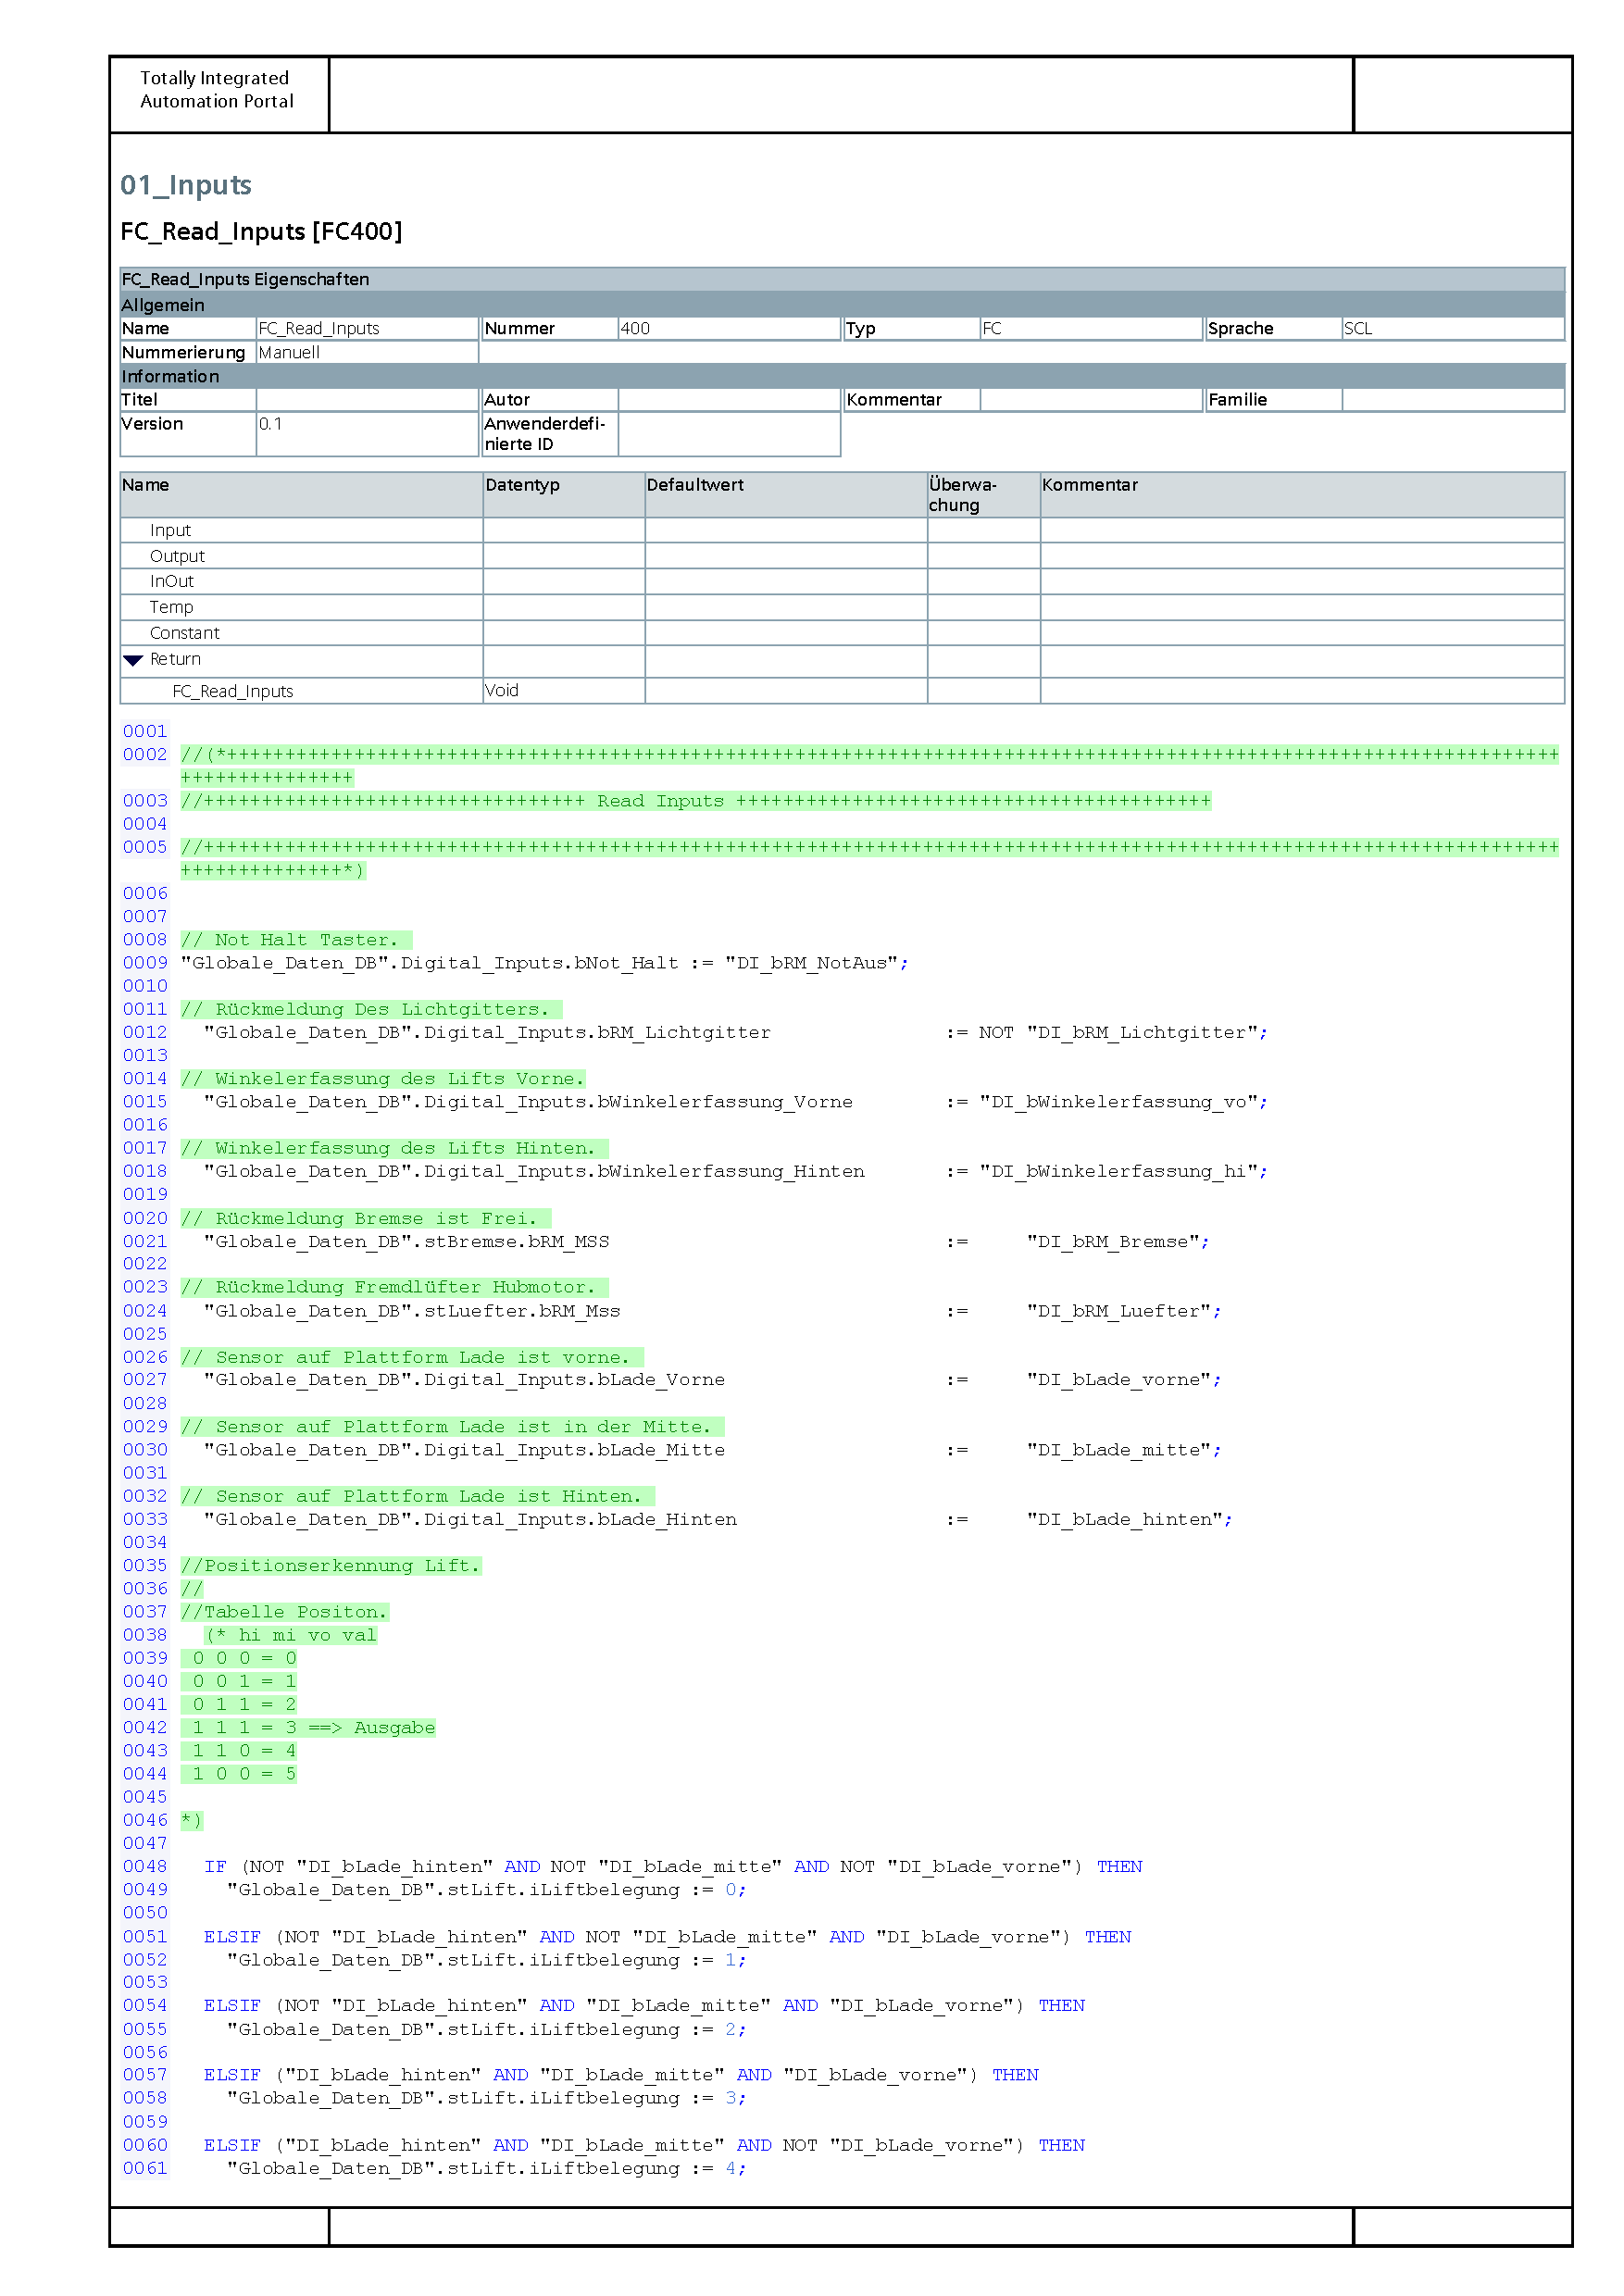
\includepdf[scale=0.8,pages=-,link=true,linkname=Inp]{../PROGRAMM/EinzelnePdfs/Inputs.pdf}
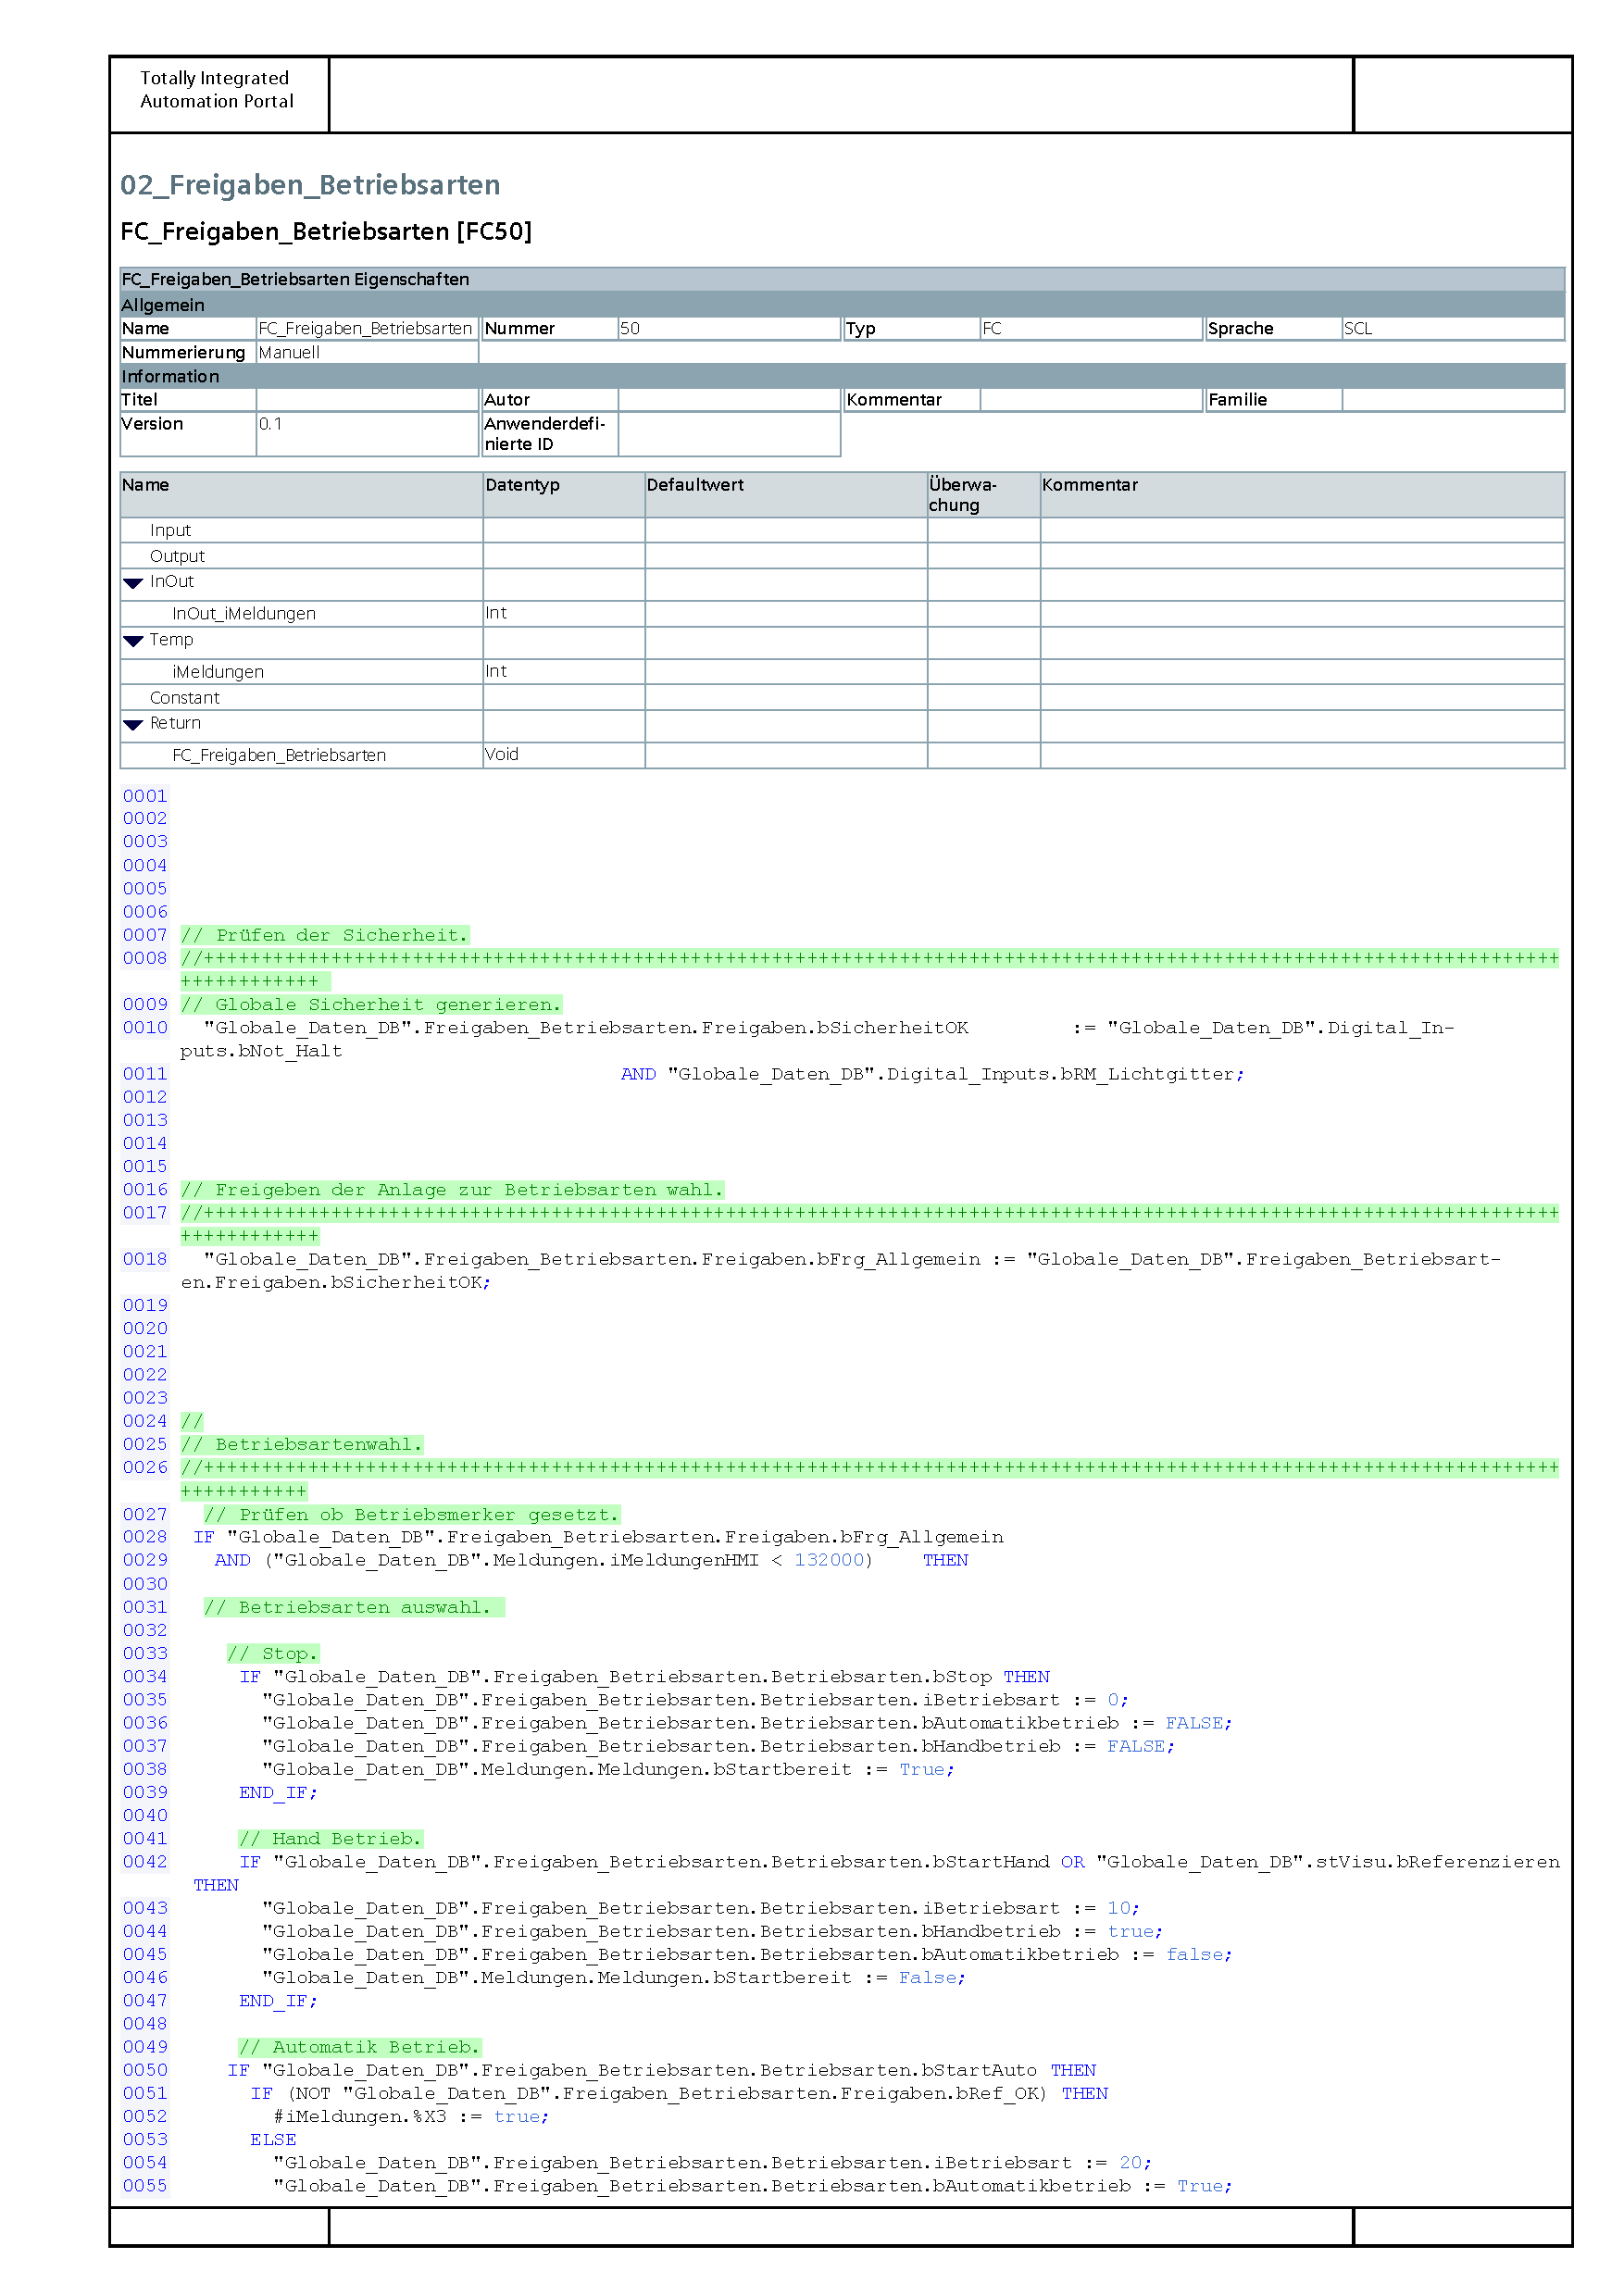
\includepdf[scale=0.8,pages=-,link=true,linkname=FrgBa]{../PROGRAMM/EinzelnePdfs/Freigaben_Betriebsarten.pdf}
%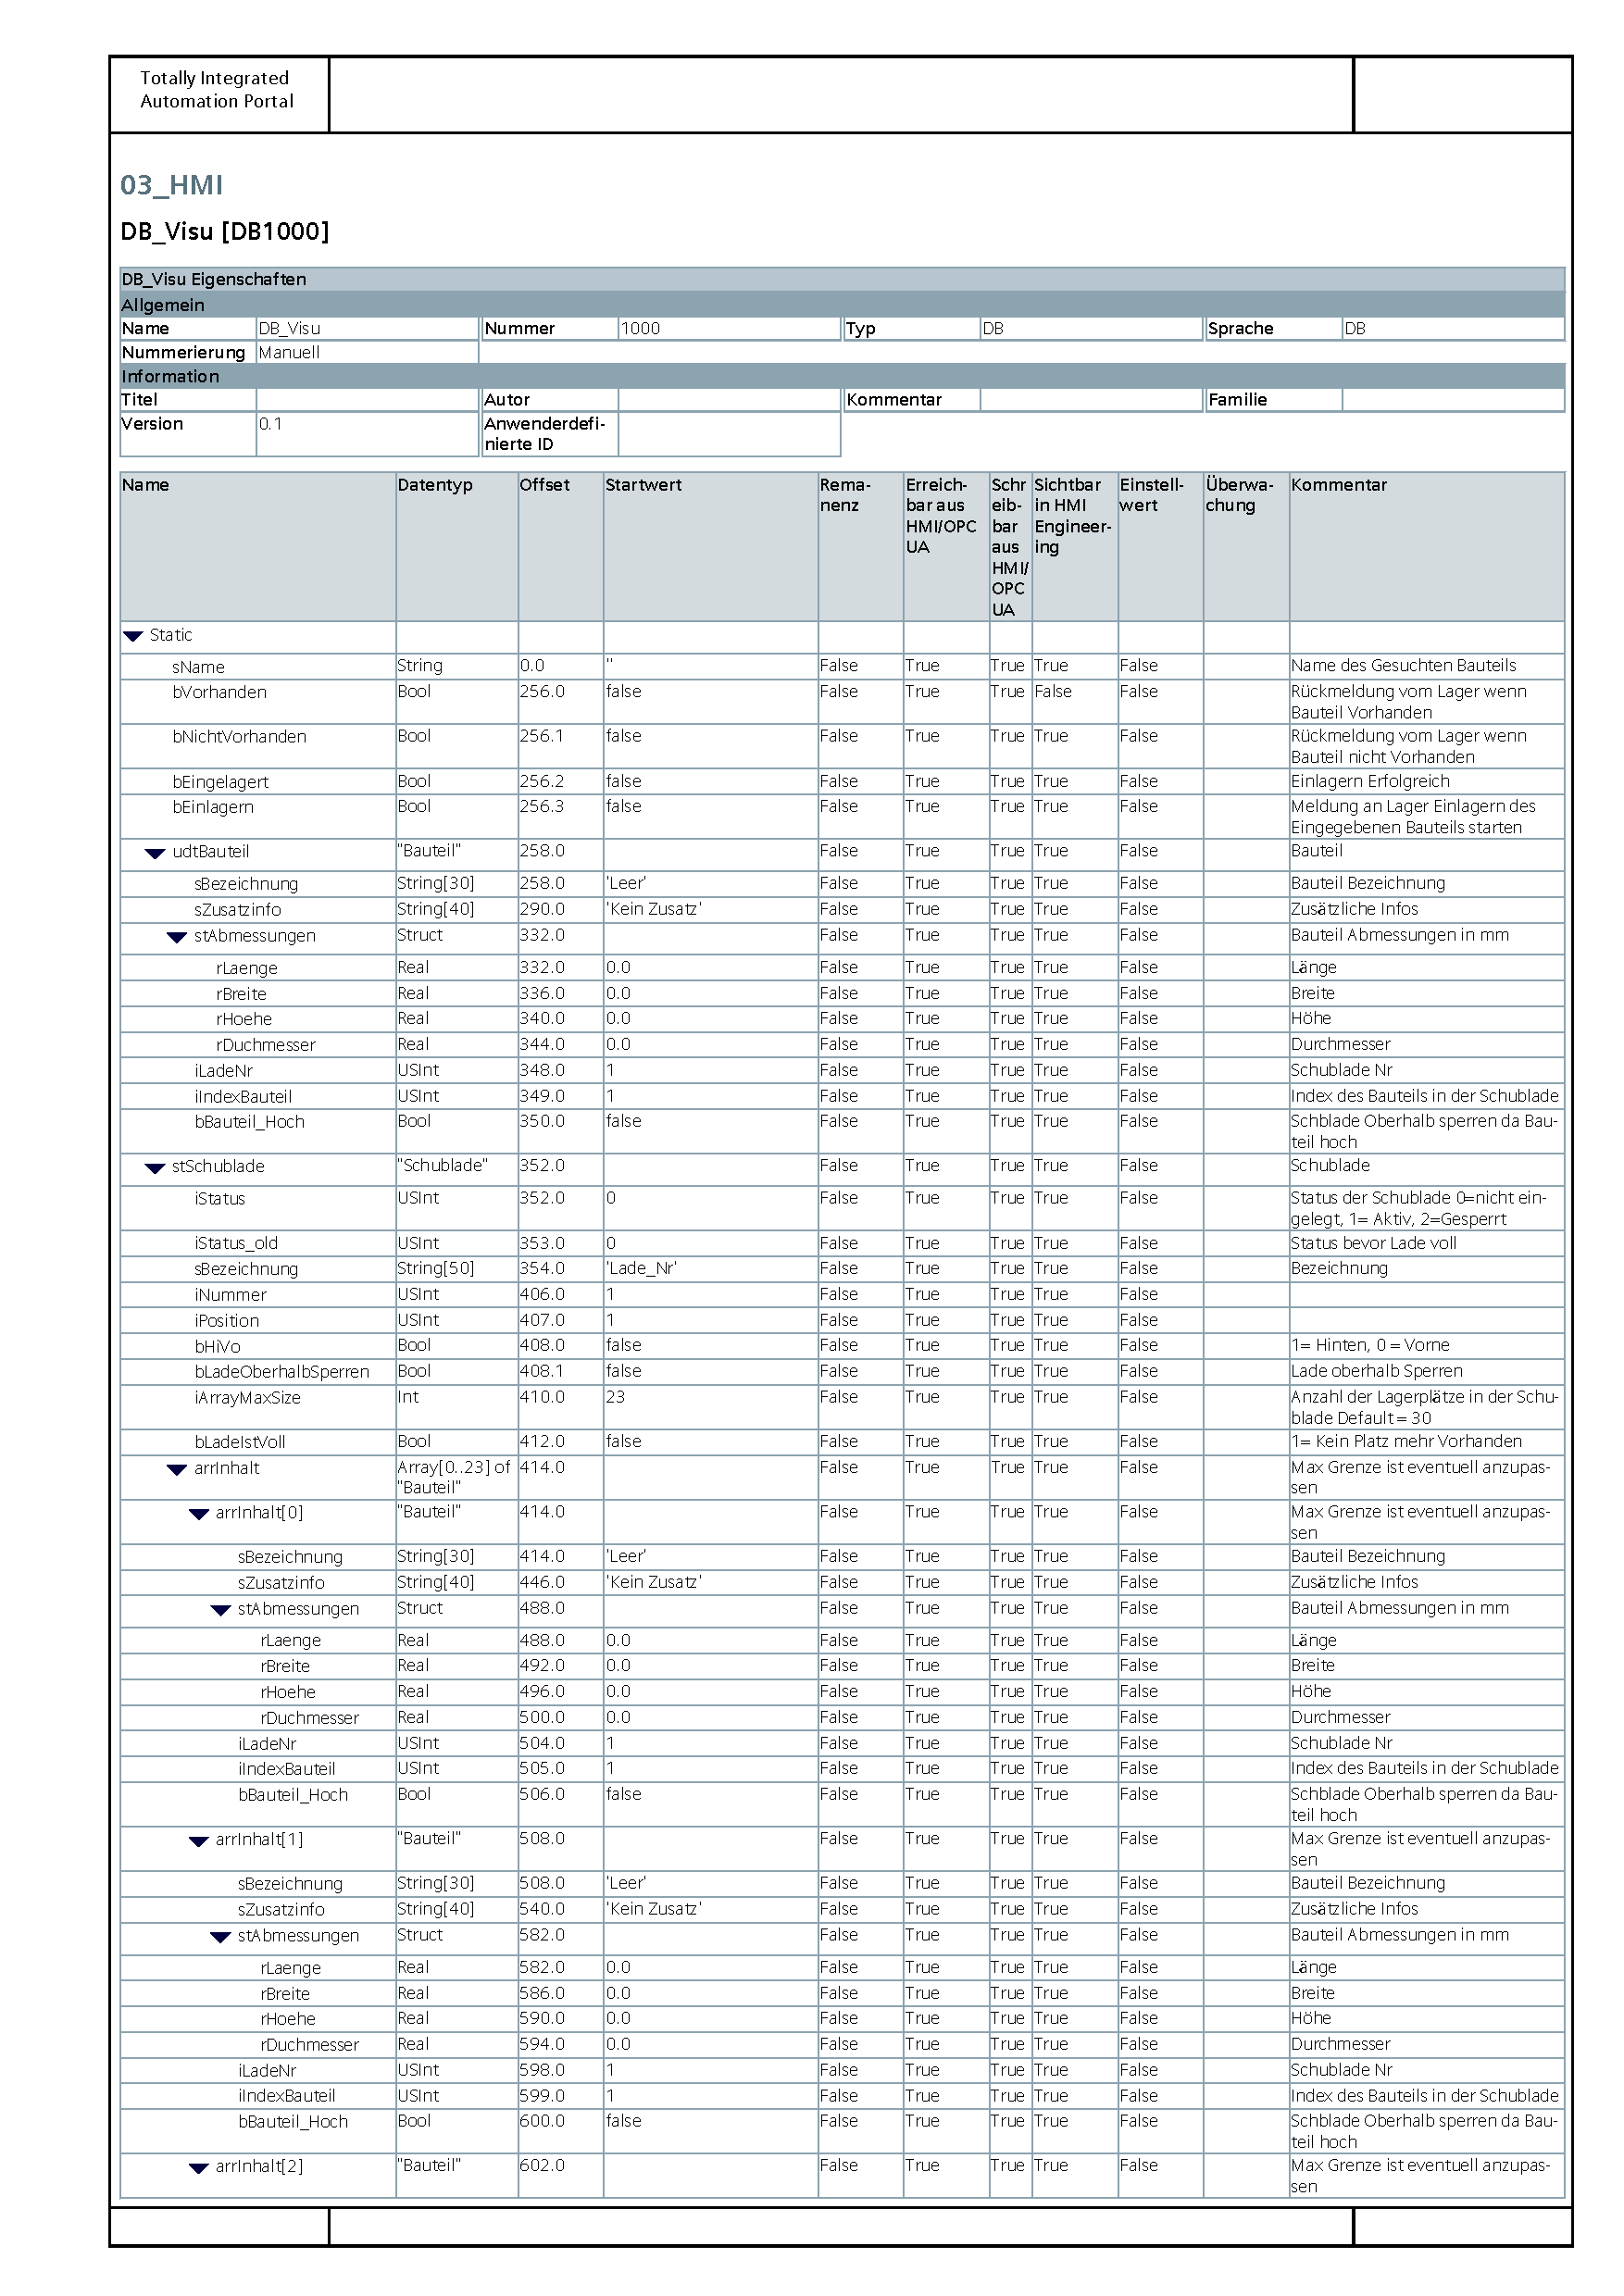
\includepdf[scale=0.8,pages=-,link=true,linkname=HMISS]{../PROGRAMM/EinzelnePdfs/HMI_Schnittstelle.pdf}
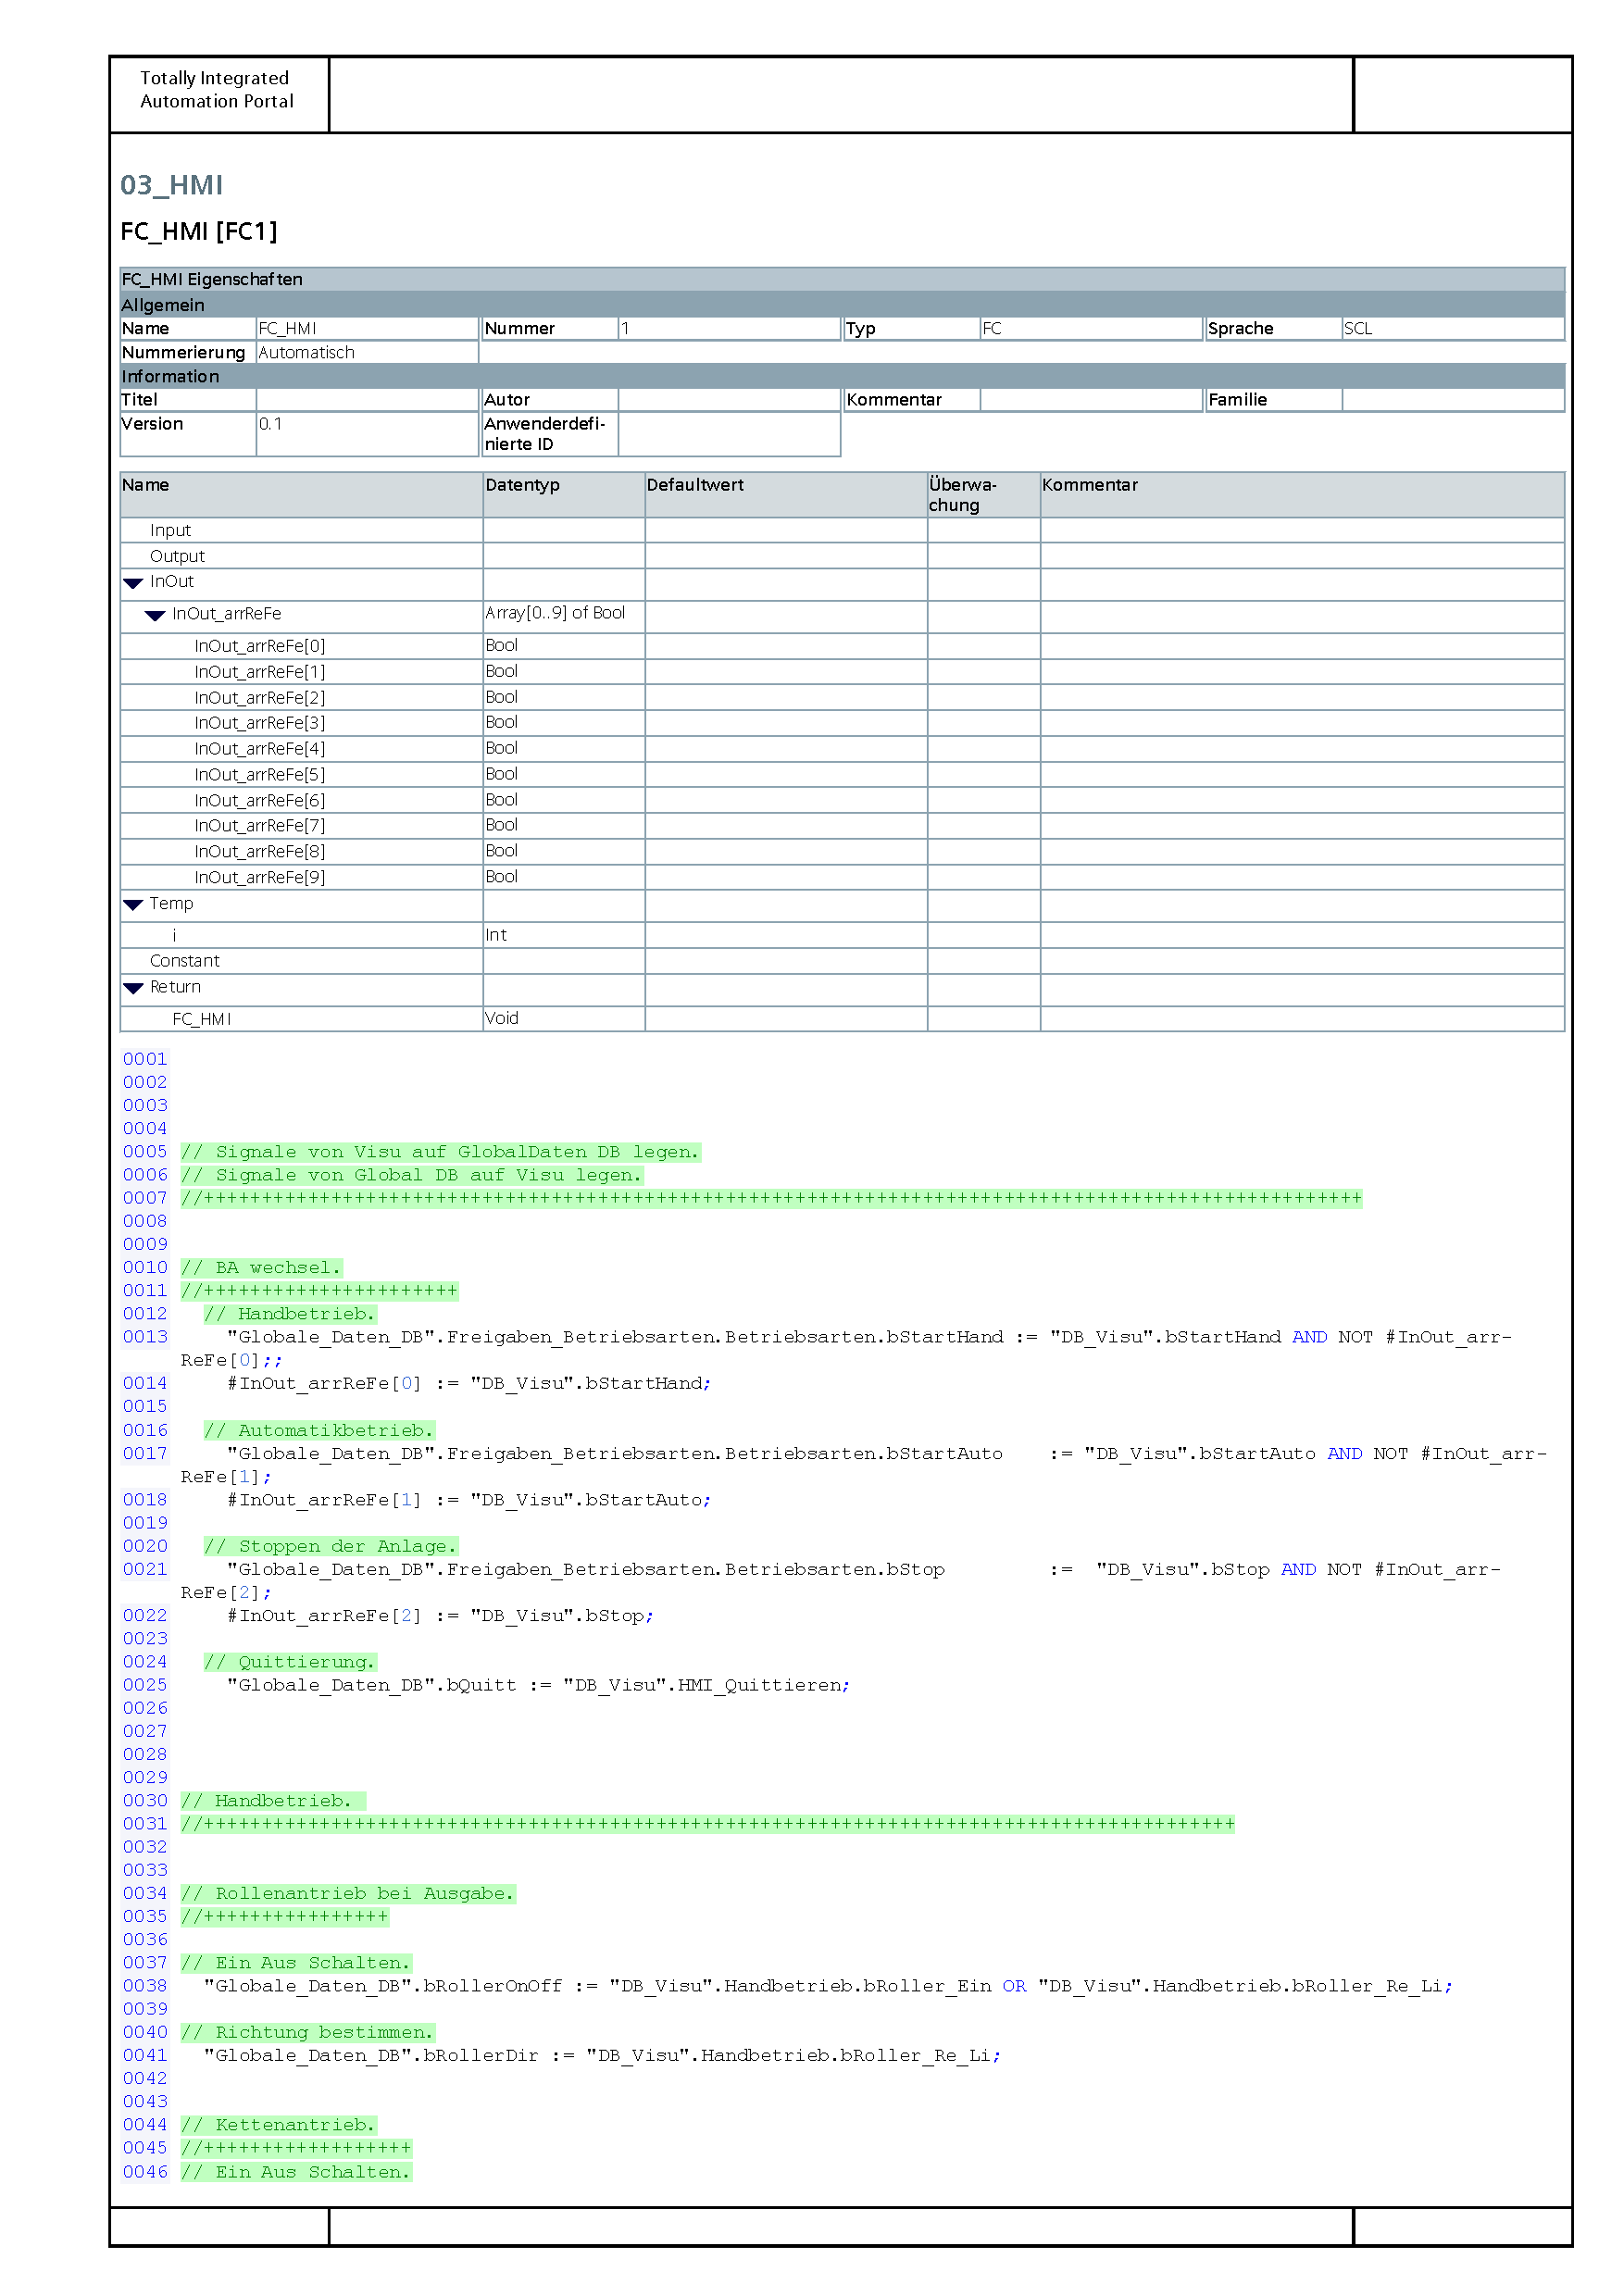
\includepdf[scale=0.8,pages=-,link=true,linkname=HMI]{../PROGRAMM/EinzelnePdfs/HMI.pdf}
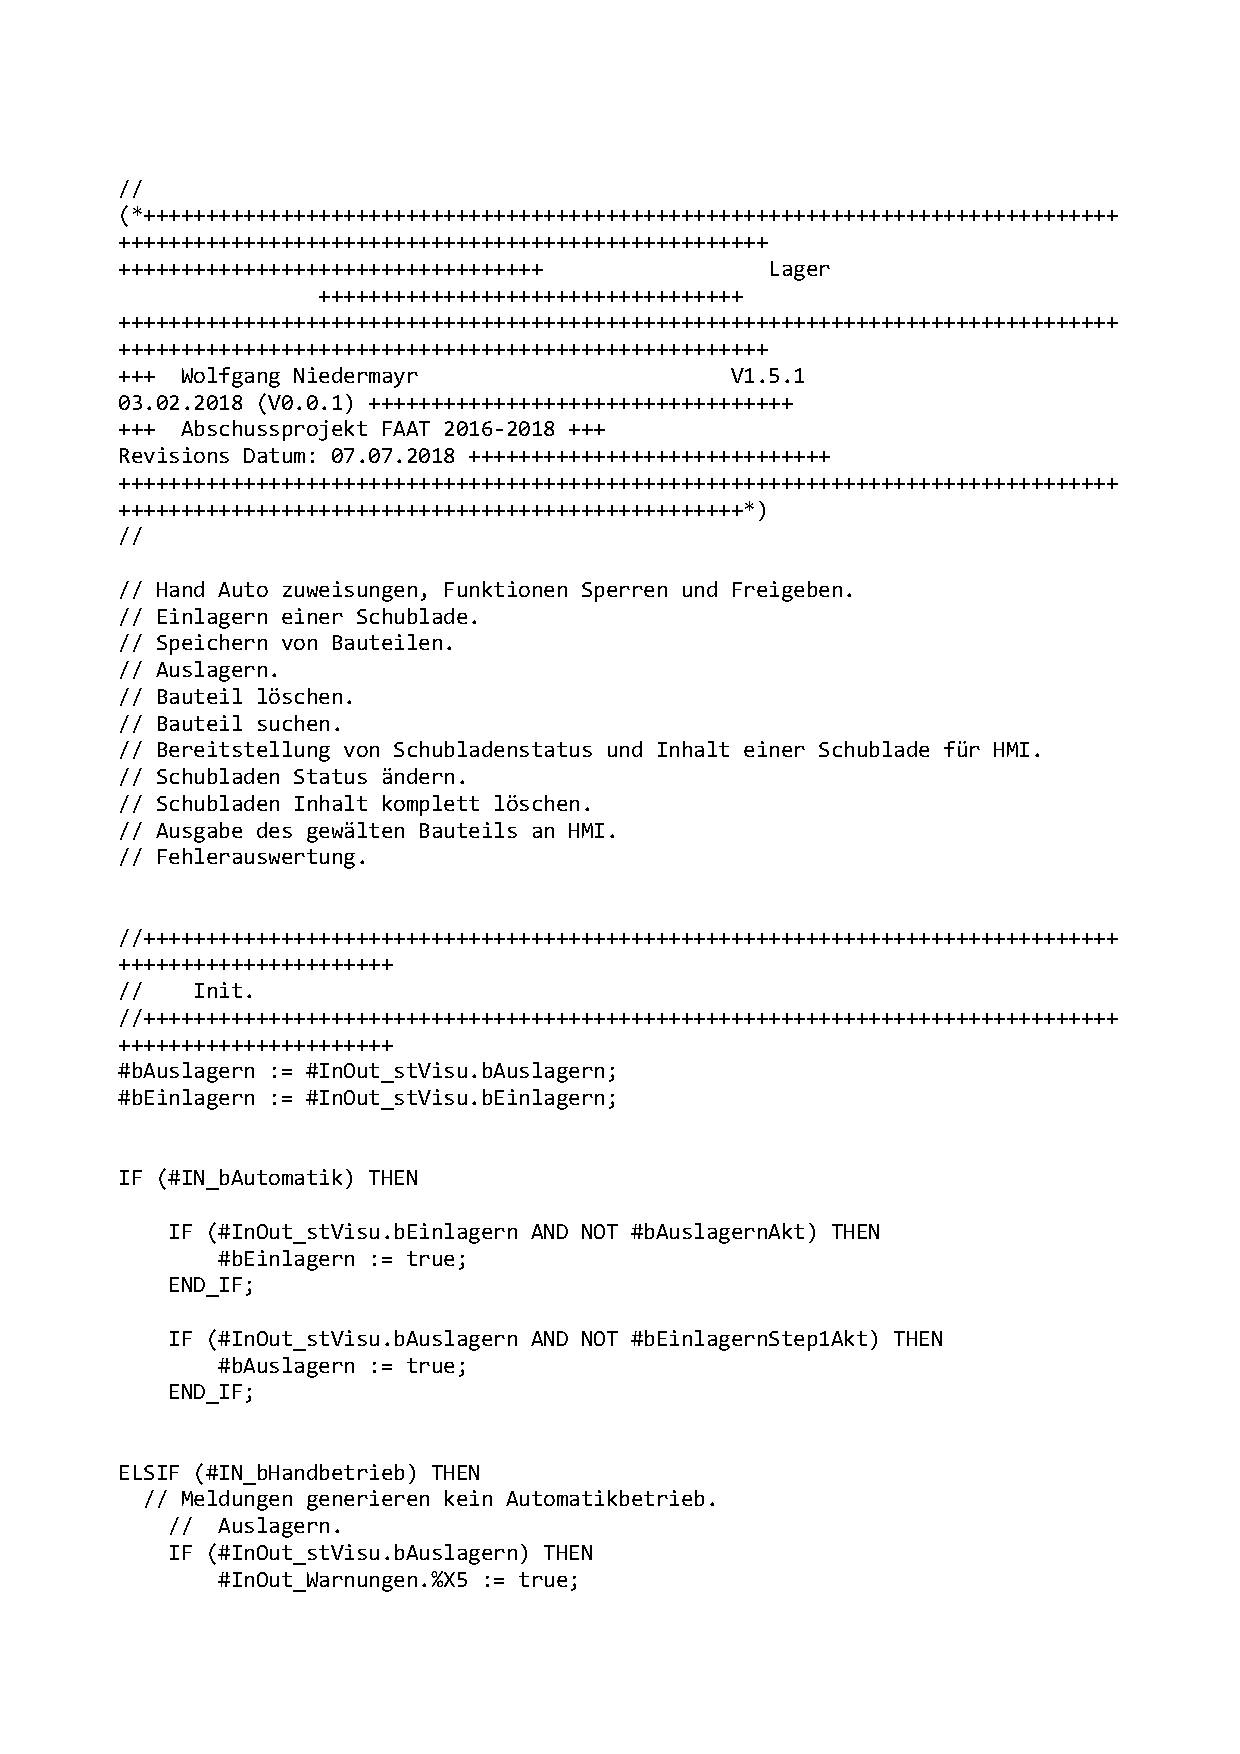
\includepdf[scale=0.8,pages=-,link=true,linkname=Lager]{../PROGRAMM/EinzelnePdfs/Lager.pdf}
%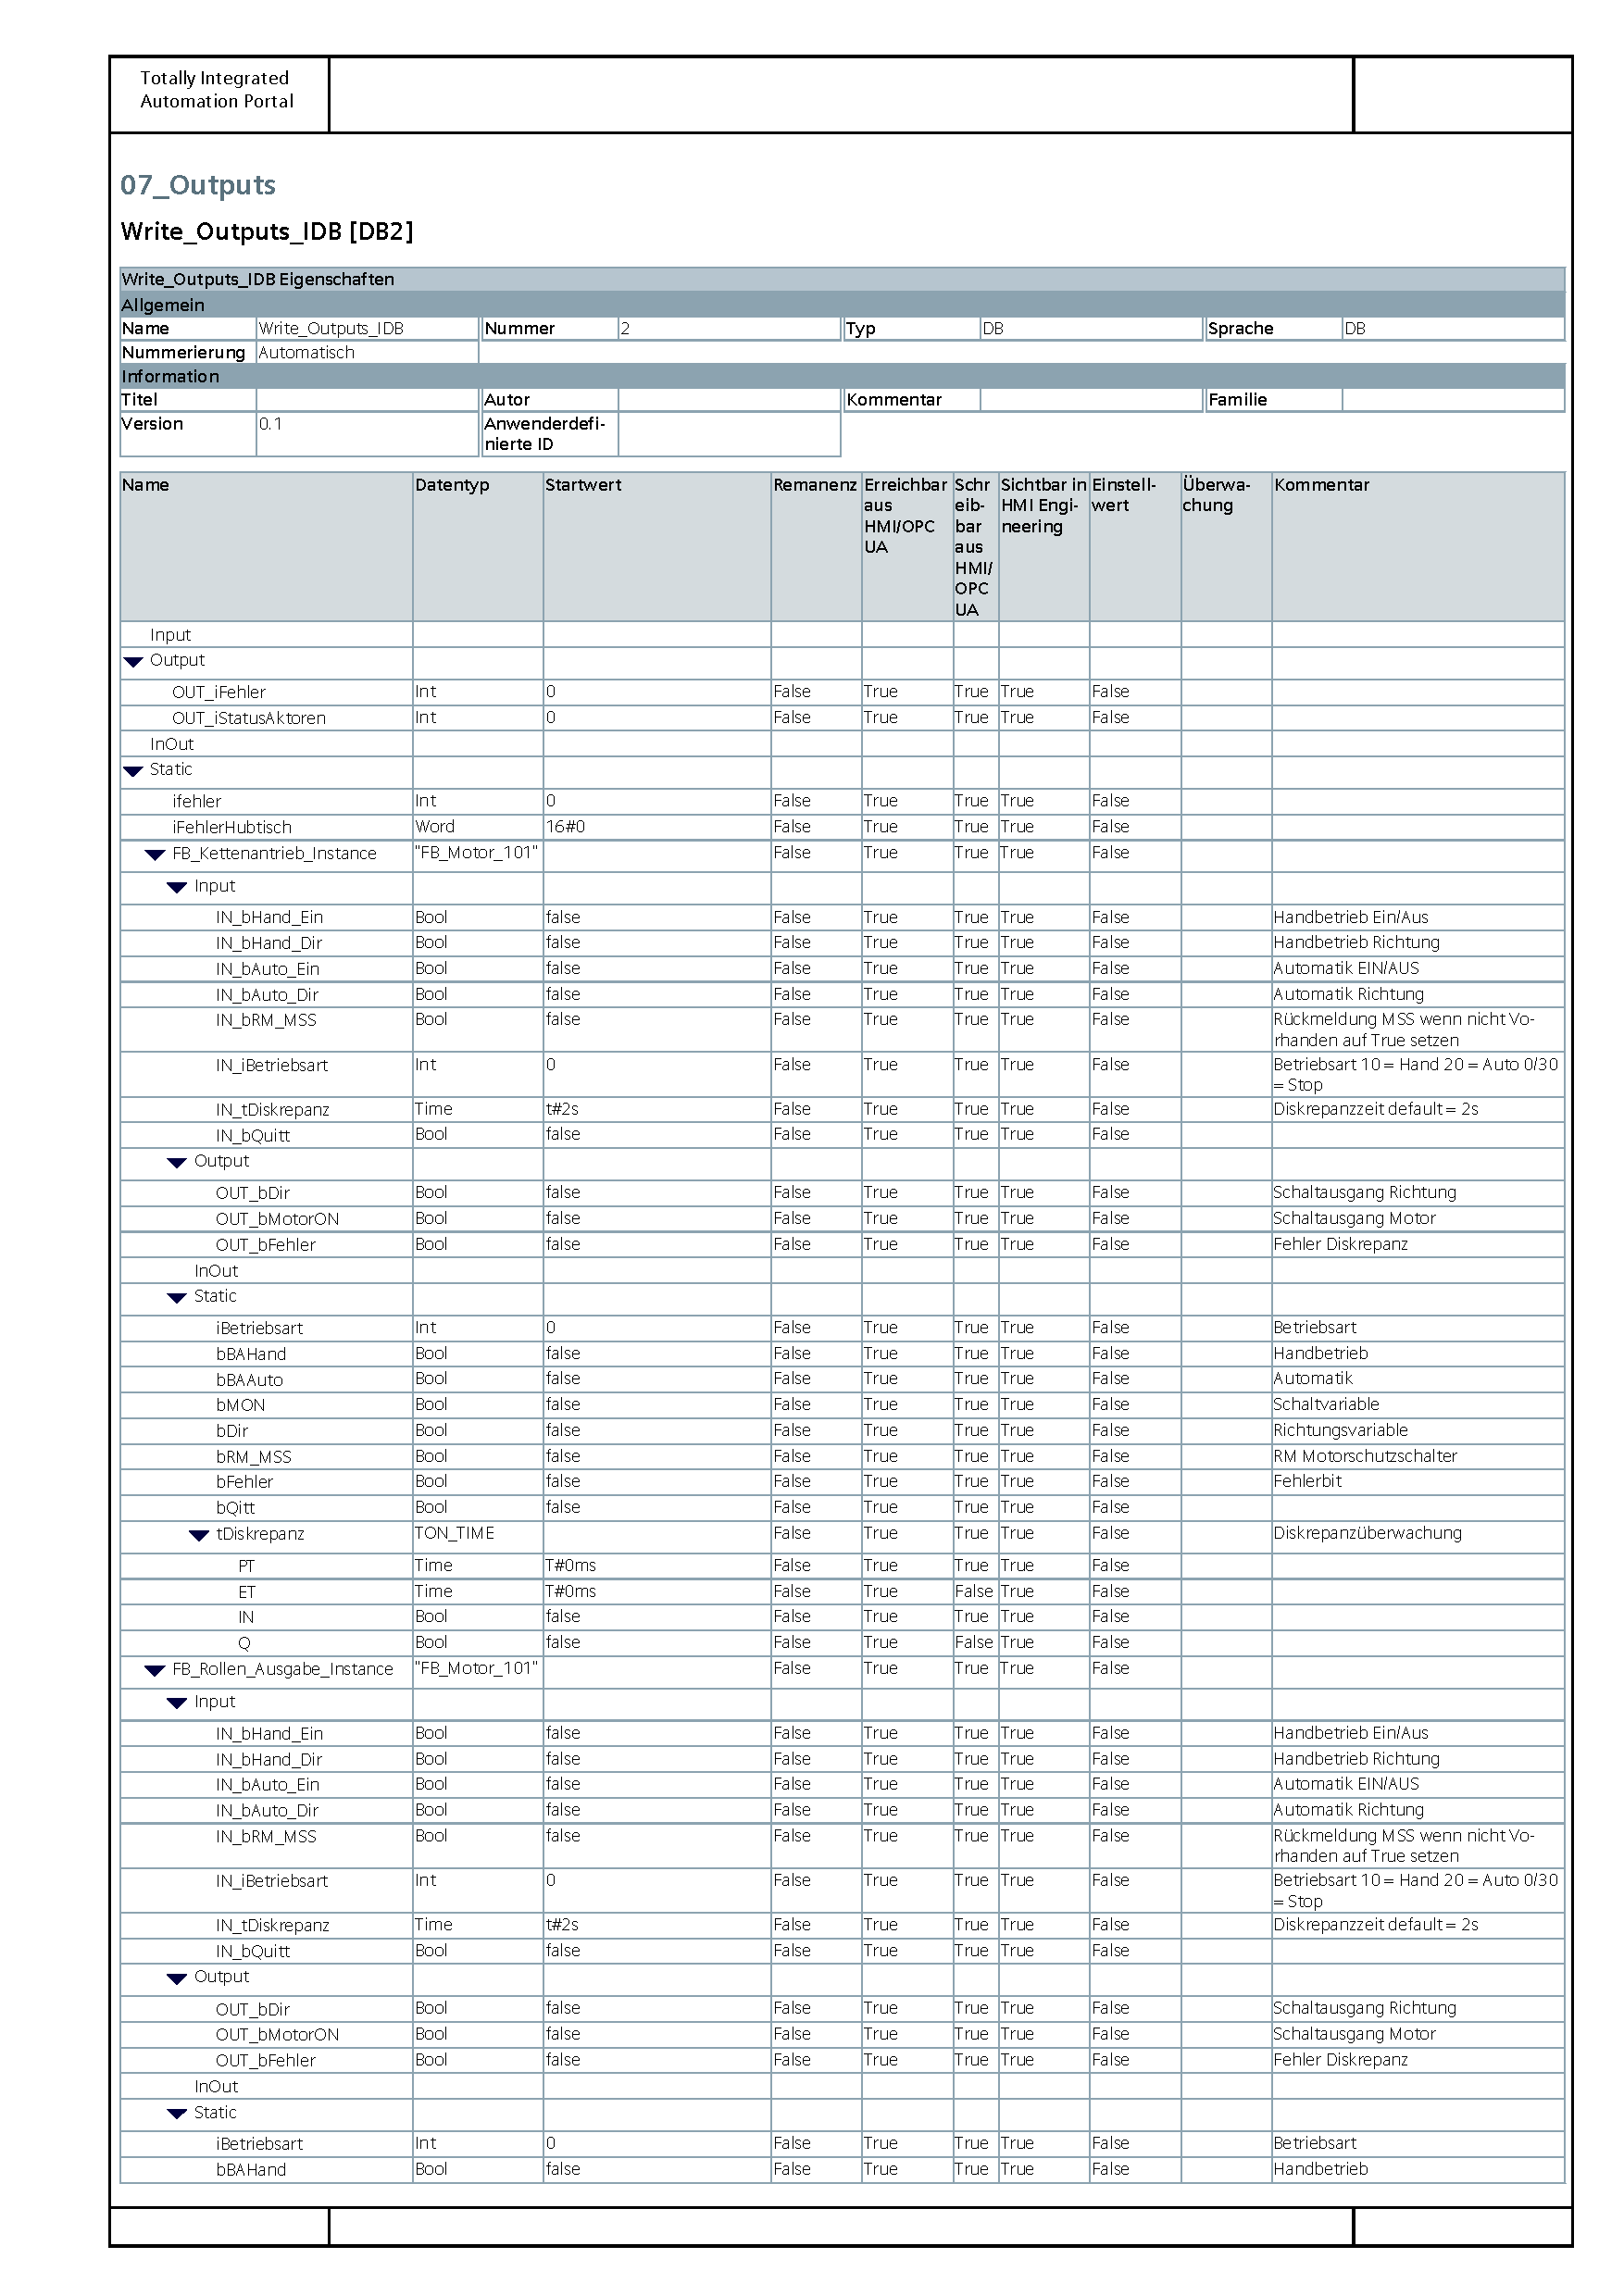
\includepdf[scale=0.8,pages=-,link=true,linkname=OutSS]{../PROGRAMM/EinzelnePdfs/Outputs_Schnittstelle.pdf}
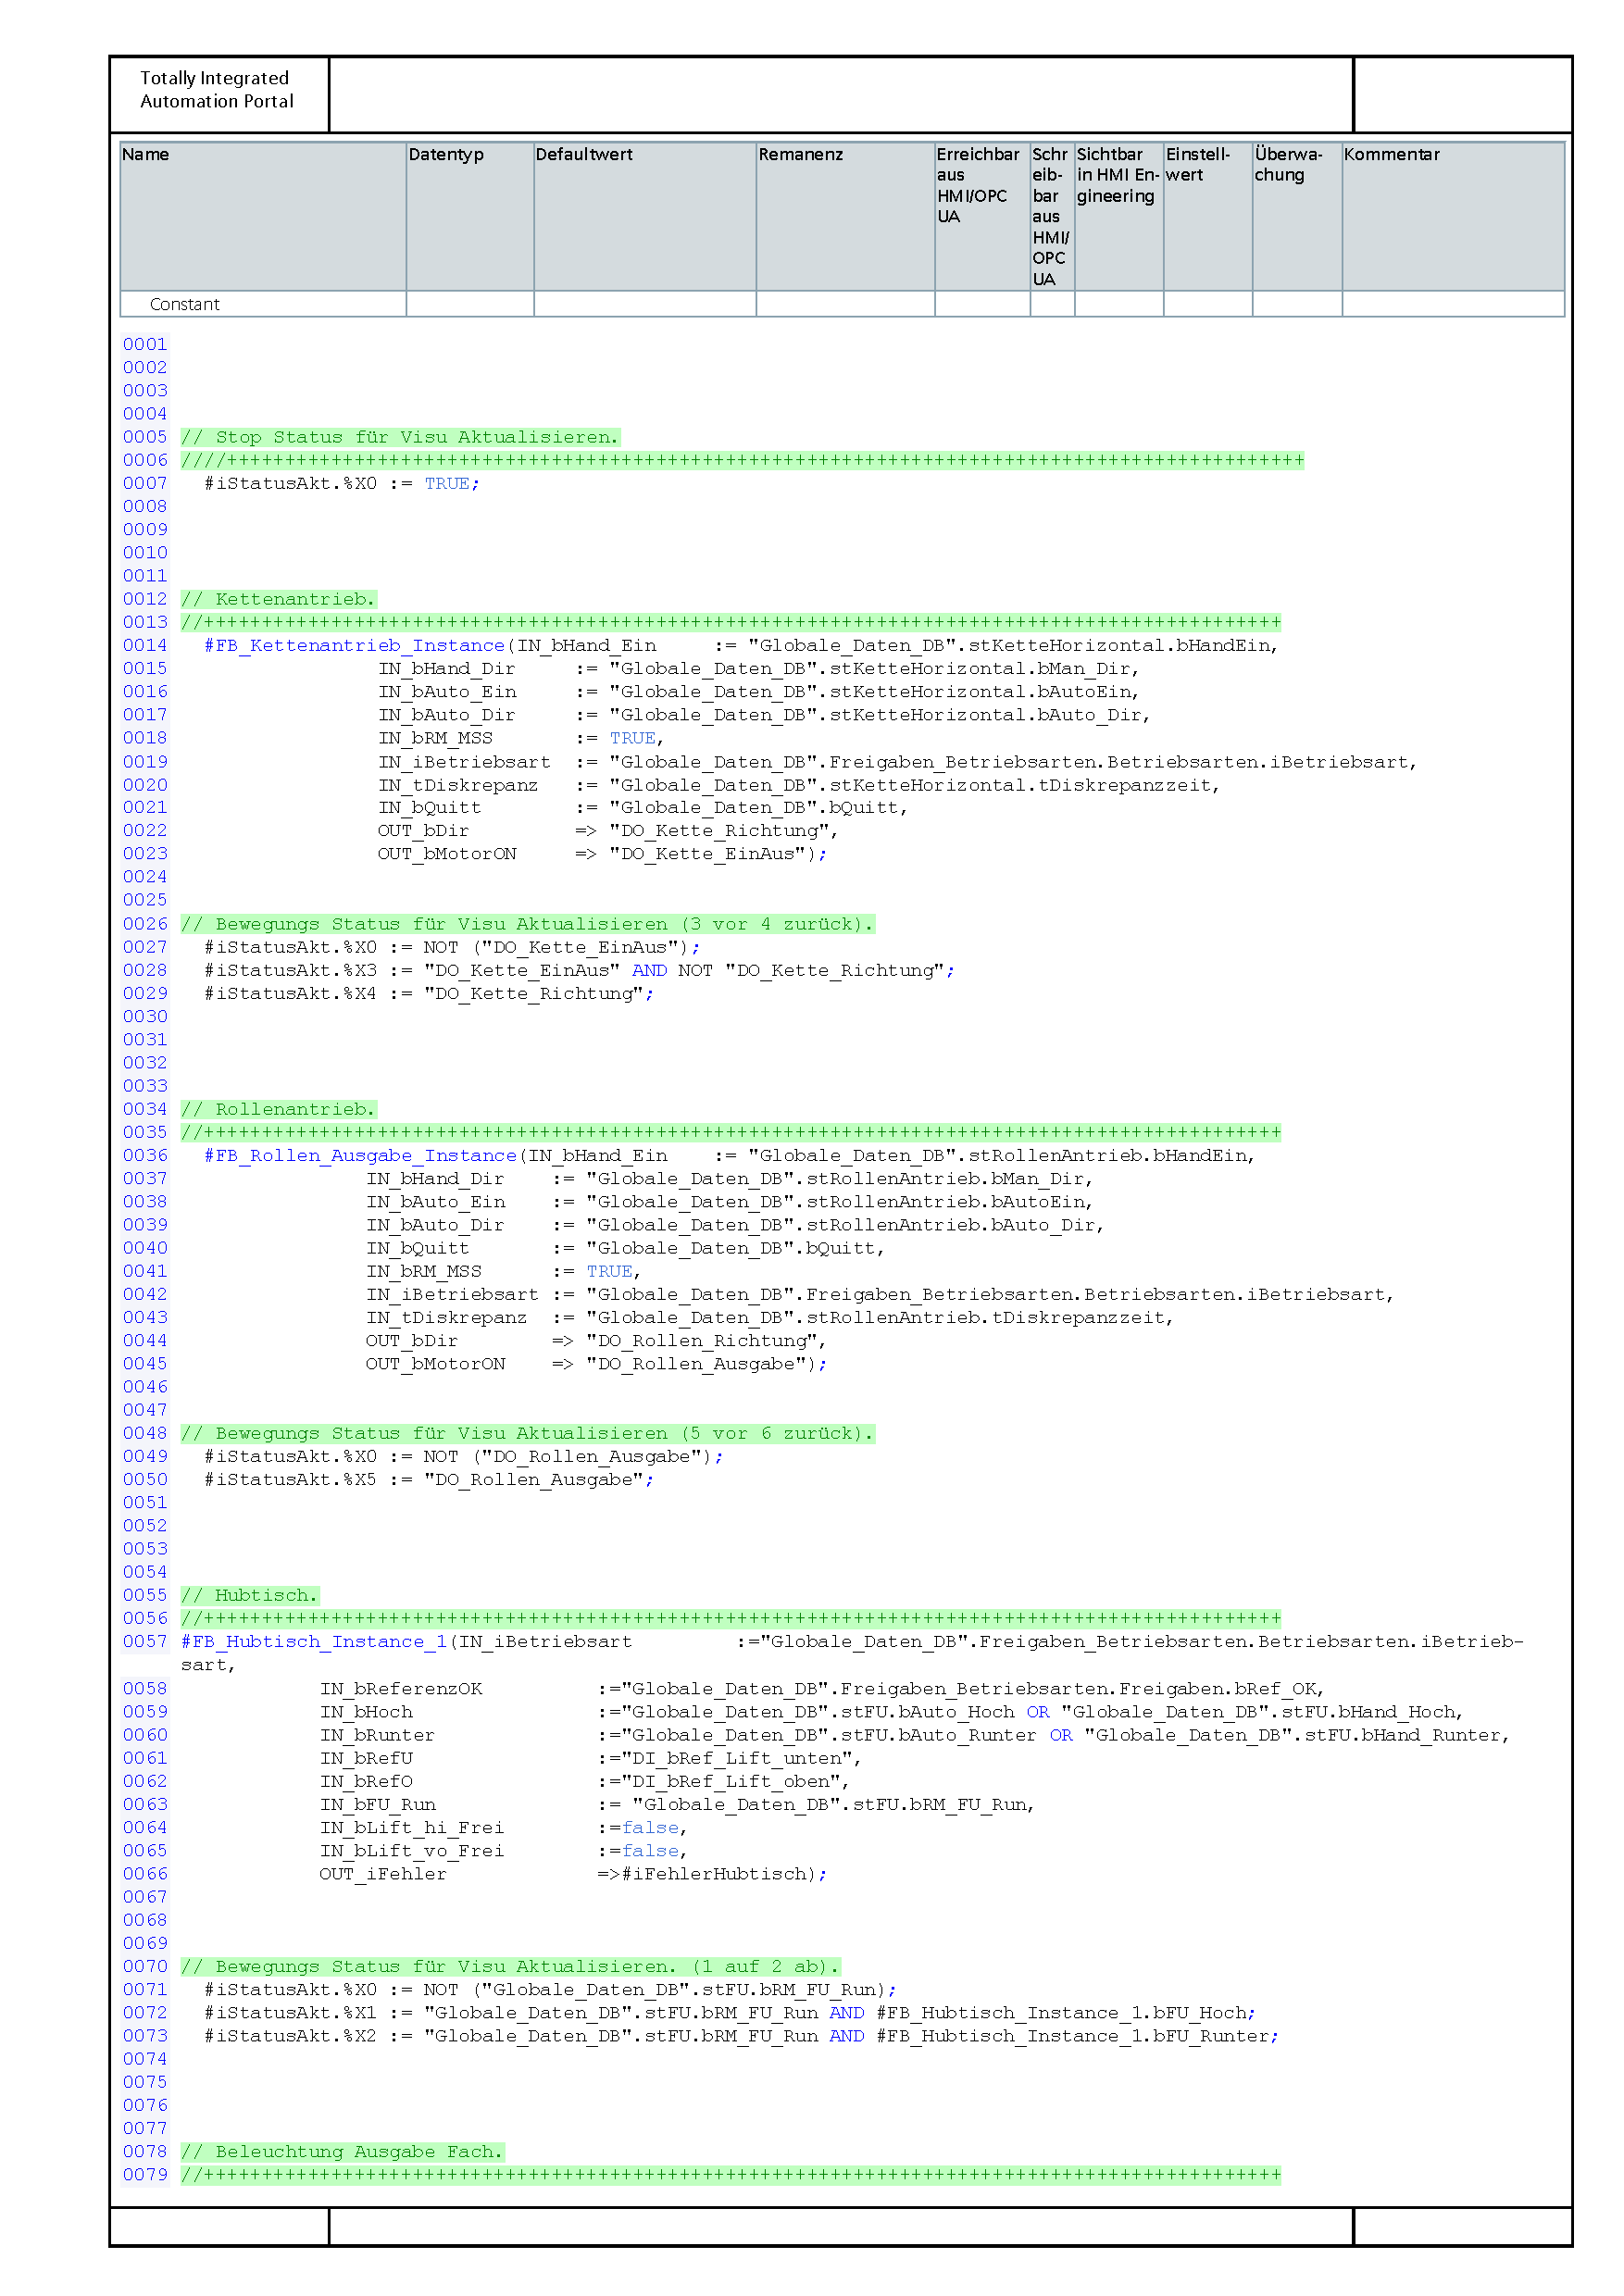
\includepdf[scale=0.8,pages=-,link=true,linkname=Out]{../PROGRAMM/EinzelnePdfs/Outputs.pdf}
\end{document}